\documentclass[10pt,reqno]{beamer} 

\usepackage{listings} 
\usepackage{array} 
\usepackage{graphicx} 
\usepackage{lineno} 
\usepackage{dcolumn} 
\usepackage{bm} 
\usepackage{color} 
\usepackage{overpic} 
\usepackage{multirow} 
\usepackage[english]{babel} 

\newcommand{\mup}{\mu^{+}} 
\newcommand{\mum}{\mu^{-}} 

\usetheme{Warsaw} 
\setbeamertemplate{footline}[frame number]
\begin{document} 

\begin{frame} 

\title{Search for an extra higgs decaying to $\mup\mum$}
\author{\underline{XYZ}, ABC \\ some insitute}
\titlepage

\end{frame}

\begin{frame} 



\frametitle{Content}



\begin{enumerate}
\item Introduction
\item Some models
\item Summary
\end{enumerate} 



\end{frame} 

\begin{frame} 



\frametitle{introduction~\label{intro}}



Why an extra higgs needed?

\begin{itemize}
\item Fermion mass hierarchy
\item Dark matter candidate
\item other
\end{itemize} 



\begin{figure}[htbp] 
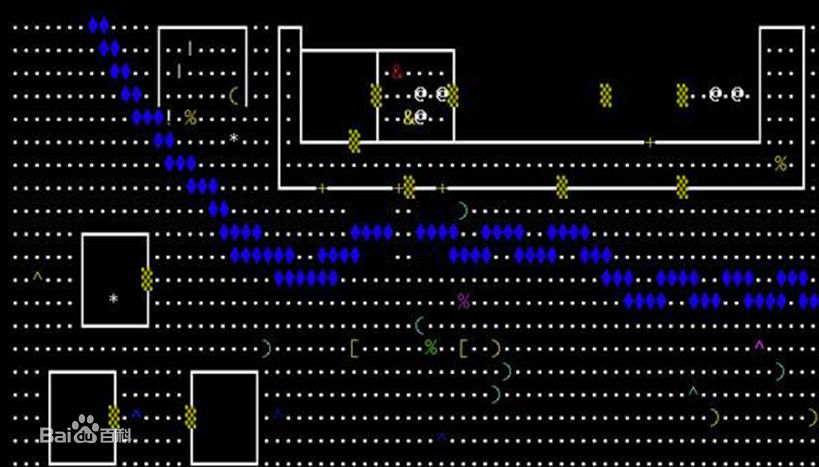
\includegraphics[width =0.5\textwidth]{fig/nethack.jpg} 
\end{figure} 



\end{frame} 

\begin{frame} 



\frametitle{some models}



\begin{enumerate}
\item Standard Model: only one higgs (CP even)
\item SuperSymmetry Models: ...
\item 2-Higgs-Doublet Models (2HDM): ...
\end{enumerate} 



\begin{table}\begin{tabular} {lll} 
 \hline\hline 
 model & description \\ 
\hline
 SM & one higgs \\ 
 SUSY & explain to fermion mass hierarchy \\ 
 2HDM & predict big FCNCs \\ 
\hline\hline 
 \end{tabular}\end{table} 





\end{frame} 

\begin{frame} 



\frametitle{Summary~\label{summary}}



\begin{enumerate}
\item No extra higgs is found for the moment ...
\end{enumerate} 





\end{frame} 

\end{document}

